% !TeX program = xelatex
\documentclass[12pt, a4paper]{article}
\usepackage{xltxtra}

% ! Language and fonts !
\usepackage{polyglossia}
% language
\setmainlanguage{russian}
\setotherlanguage{english}
% fonts
\setmainfont[Ligatures=TeX]{CMU Serif}
\setromanfont[Ligatures=TeX]{CMU Serif} 
\setsansfont[Ligatures=TeX]{CMU Serif} 
\setmonofont[Ligatures=TeX]{CMU Serif} 
% set fonts to cyrillic
\newfontfamily{\cyrillicfont}[Ligatures=TeX]{CMU Serif}
\newfontfamily{\cyrillicfontrm}[Ligatures=TeX]{CMU Serif}
\newfontfamily{\cyrillicfonttt}[Ligatures=TeX]{CMU Serif} 
\newfontfamily{\cyrillicfontsf}[Ligatures=TeX]{CMU Serif} 
% rename pictures and tables
\addto\captionsrussian{
  \renewcommand{\figurename}{Рис.}
  \renewcommand{\tablename}{Табл.}
}
% math
\usepackage{unicode-math}
\setmathfont{TeX Gyre Termes Math}

% ! Document format !
\usepackage{comment}
\begin{comment}]
\usepackage{geometry} % Задаём поля:
\geometry{left=3cm} % левое — 3 см;
\geometry{right= 1.5cm} % правое — 1,5 см;
\geometry{top=2cm} % верхнее — 2 см;
\geometry{bottom=2cm} % нижнее — 2 см;
\usepackage{setspace} \onehalfspacing % Задаём «полуторный» межстрочный интервал.
\usepackage{indentfirst} % Автоматически добавляем отступ в каждый новый абзац.
\usepackage[all]{nowidow} % Пакет для борьбы с «висячими» строками абзацев, лучшая альтернатива переопределению \clubpenalty и \widowpenalty.
\usepackage{enumitem} % Настраиваем работу со списками:
\def\labelitemi{—} % задаём длинное тире как стандартный маркер ненумерованного списка;
\setlist{nolistsep} % убираем дополнительные отступы между элементами списка;
\usepackage{fancyhdr} % Настраиваем колонтитулы:
\pagestyle{fancy} % задаём макет страницы, отличный от стандартного;
\fancyhf{} % сбрасываем содержимое колонтитулов;
\renewcommand{\headrulewidth}{0pt} \renewcommand{\footrulewidth}{0pt} % убираем декоративные линии из колонтитулов;
\fancyfoot[C]{\thepage} % настраиваем расположение номера страницы в нижнем колонтитуле: L — слева, R — справа, C — по центру.
\addto\captionsenglish{\renewcommand{\partname}{}} % меняем имя главы
\setcounter{part}{-\maxdimen} % убираем счет глав
\usepackage{titlesec} % настраиваем заголовки частей документа:
\titleformat*{\section}{\newpage\normalsize\bfseries\centering} % настраиваем заголовок раздела; начинаем каждый раздел с новой страницы; размер шрифта — такой же, как во всем документе, начертание — полужирное, выравнивание  — по центру.
\end{comment}

% ! useful package !
\setlength{\mathsurround}{2pt}
\usepackage{mathtext}
\usepackage{booktabs,tabulary,tabularx,longtable}
\newcolumntype{M}[1]{>{\centering\arraybackslash}m{#1}} % resize row
\newcolumntype{N}{@{}m{0pt}@{}} % zero row
\usepackage{array} % for extrarowheight
\usepackage{varwidth} % for the varwidth minipage environment
\usepackage{graphicx} 
\usepackage{listings} 
\usepackage{color} 
\usepackage{xunicode}
\usepackage{ulem}

\usepackage{sectsty}

\allsectionsfont{\centering}
\setcounter{secnumdepth}{0}

\usepackage{multicol}
\usepackage{lipsum}
\usepackage{mwe}
\usepackage{float}
\usepackage{rotating}

\usepackage[left=2cm,right=2cm,top=2cm,bottom=2.5cm]{geometry}

\author{Круглов Иван} 
\title{\textbf{Инструмент управления временем и задачами - Joplin}} 
\date{25 сентября 2022 г.} 

\begin{comment}
\addto\captionsrussian{
  \renewcommand{\contentsname}
    {Мы будем исследовать такие функции как}
}
\end{comment}

\begin{document}

    % page 1
    \begin{Huge}
        \maketitle
    \end{Huge}
    \null
    \vfill
    \begin{turn}{-45} 
        \Huge{Сверстано в \XeLaTeX}
    \end{turn}
    

    % page 
    \newpage
    \tableofcontents

    %page
    \newpage
    \section{Общий обзор}
    \subsection{Общий вид}
    Joplin является скорее средством для заметок, однако именно поэтому его очень удобно
    использовать как средством управления задачами и временем.
    Основной функционал Joplin очень похож на функционал Notion или Trello.
    Здесь так же есть:
    \begin{itemize}
        \item Возможность создать различные рабочие пространства
        \item В каждом пространстве можно создать задачу/заметку
        \item Заметка редактируется в формате markdown и в реальном времени мы можем видеть результат
    \end{itemize}
    Общий вид выглядит следующим образом

    \begin{figure}[H]
        \centering
        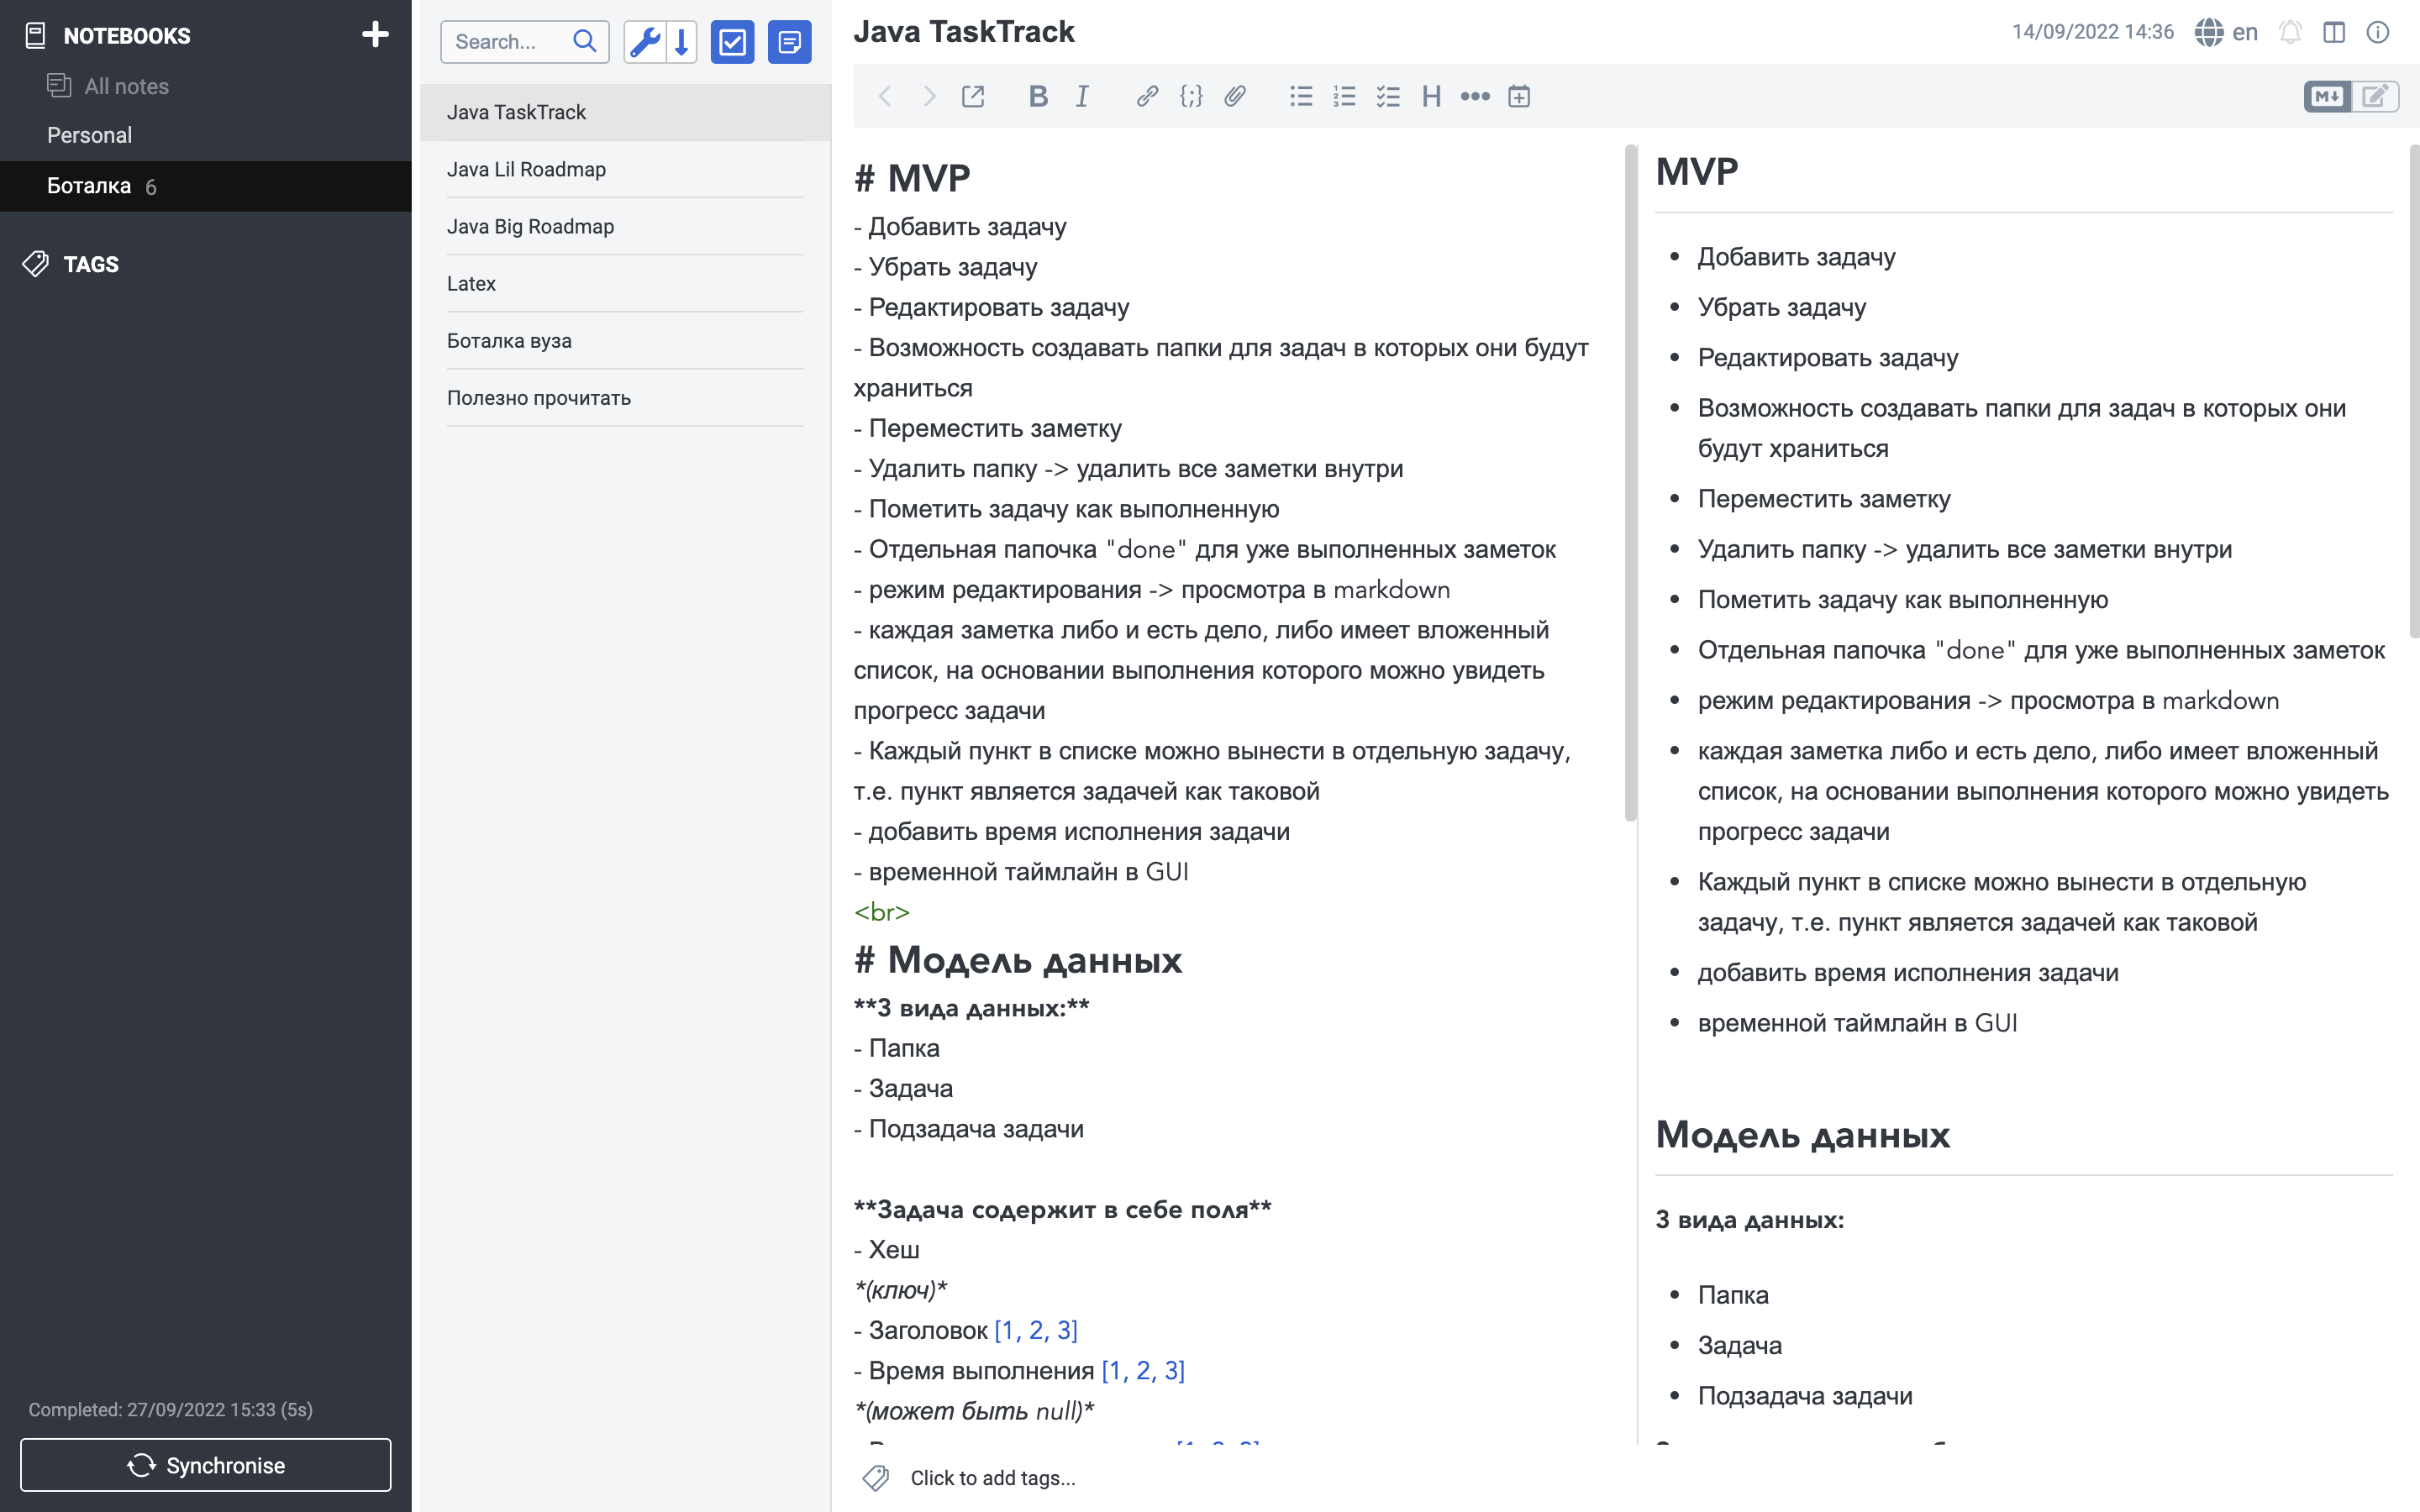
\includegraphics[width=0.95\linewidth]{src/1.png}
        \caption{Общий вид}
    \end{figure}

    А все заметки можно сортировать по тегам, а так же располагать их в требуемом порядке

    \newpage
    \subsection{Создание первой заметки}
    Давайте попробуем создать первую заметку. Для этого создадим наше рабочее
    пространство \textit{Practice}
    Как мы видим, мы можем импортировать workspace из файла, добавить эмоджи для пространства
    или же создать для нее обычное название.
    \begin{figure}[H]
        \centering
        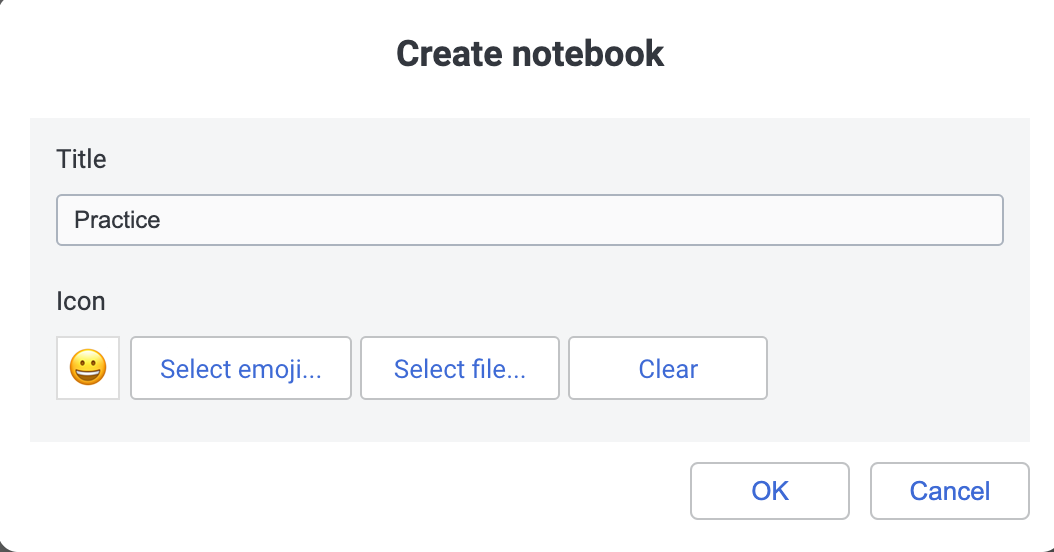
\includegraphics[width=0.75\linewidth]{src/2.png}
        \caption{Создание рабочего пространства}
    \end{figure}
    \begin{figure}[H]
        \centering
        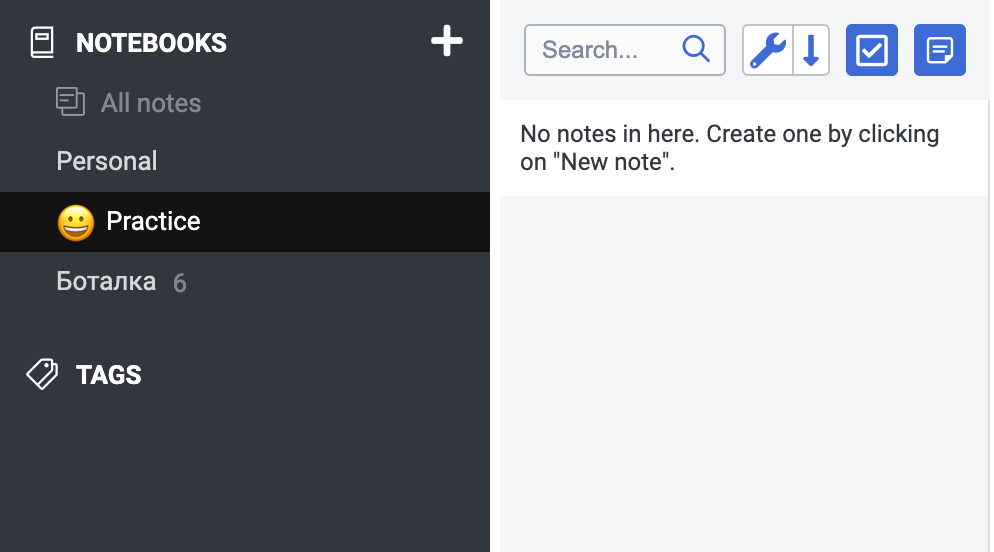
\includegraphics[width=0.75\linewidth]{src/3.png}
        \caption{Результат создания workspace \textit{(notebook)}}
    \end{figure}
    
    Далее мы создадим саму заметку, которая может быть двух видов:
    \begin{multicols}{2}

        \begin{figure}[H]
            \centering
            
\includegraphics[width=0.35\linewidth]{src/4.png}
            \caption{TODO}
        \end{figure}

    \columnbreak

        \begin{figure}[H]
            \centering
            
\includegraphics[width=0.35\linewidth]{src/5.png}
            \caption{Обычная заметка}
        \end{figure}
        
    \end{multicols}

    Особой разницы между ними нет, помимо того, что в типе заметок
    TODO их можно пометить как выполненные/невыполненные.

    \begin{figure}[H]
        \centering
        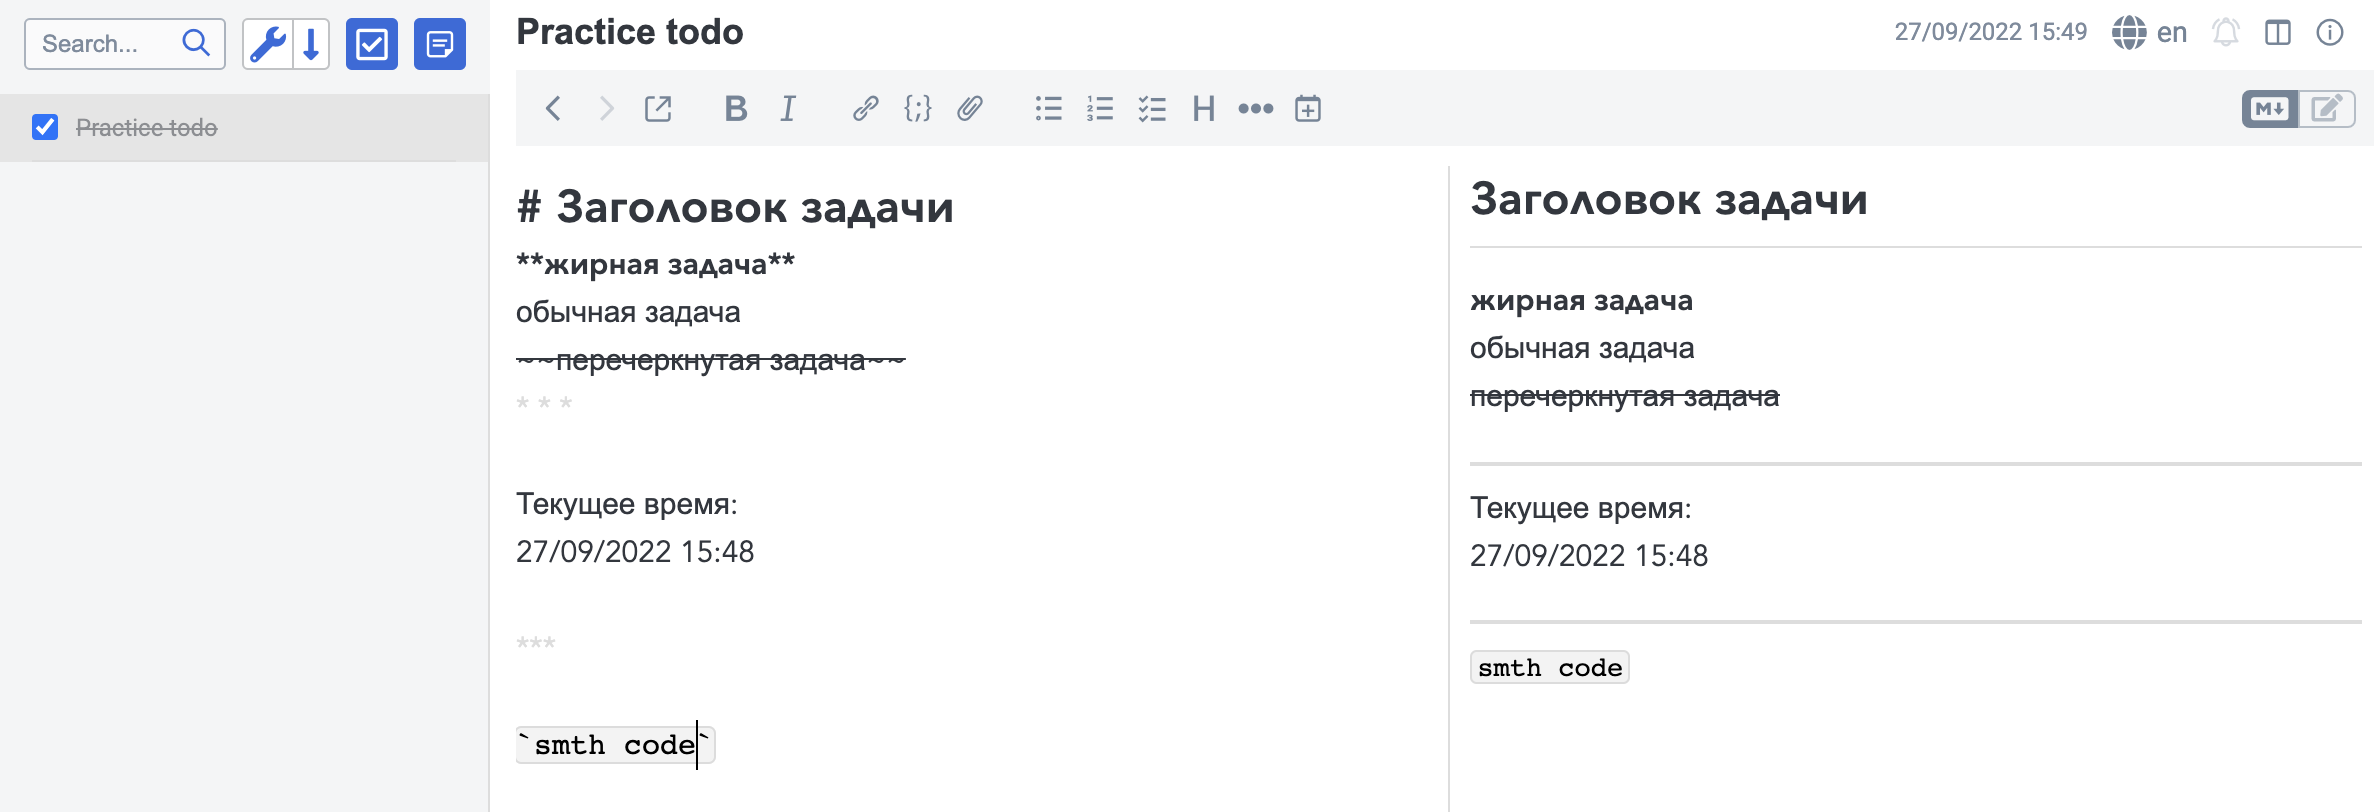
\includegraphics[width=0.9\linewidth]{src/6.png}
        \caption{Созданная TODO заметка}
    \end{figure}

    А добавив к задаче тег, мы можем просматривать задачи по разлиным тегам:
    \begin{multicols}{2}
        \begin{figure}[H]
            \centering
            
\includegraphics[width=0.75\linewidth]{src/7.png}
            \caption{Создание тега для задачи}
        \end{figure}
    \columnbreak
        \begin{figure}[H]
            \centering
            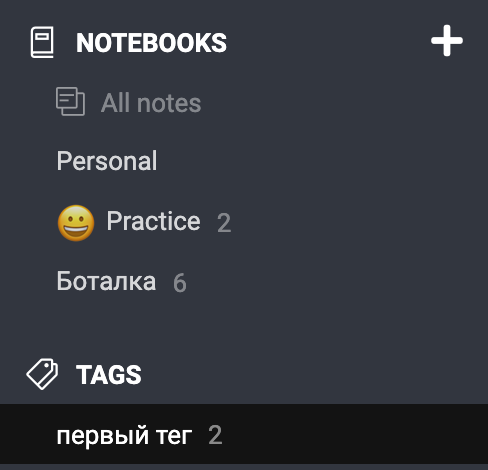
\includegraphics[width=0.75\linewidth]{src/8.png}
            \caption{Просмотр по тегу}
        \end{figure}
    \end{multicols}

    % page 
    \newpage
    \section{Основные возможности}

    Под основными возможностями мы будем подразумевать различные функции из коробки,
    которые мы можем использовать в данном инструменте\\
    Отметим также интересные плюсы:
    \begin{itemize}
        \item Вложенность хотя бы в пару уровней
        \item Простой WYSIWYG-редактор поверх markdown
        \item Возможность прикреплять файлы
        \item Автосинхронизация
        \item Работает под всеми возможными системами (или почти под всеми)
        \item Оффлайн-режим
        \item Сохранение веб-страниц
    \end{itemize}
    Функционал достаточно минималистичный, но гибкий, благодаря множественным дополнениям, которые мы рассмотрим позже
    Базовый же функционал позволяет нам:
    
    Прикрепить ссылку
    \begin{figure}[H]
        \centering
        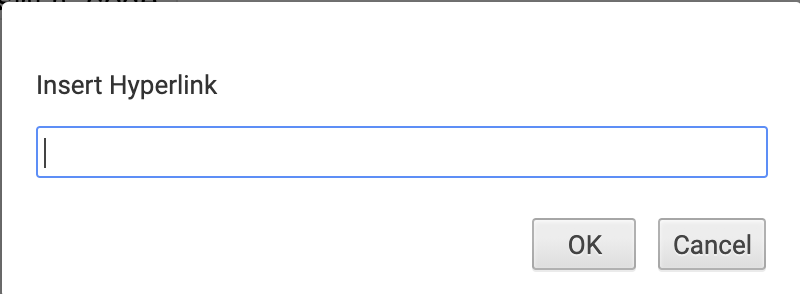
\includegraphics[width=0.75\linewidth]{src/9.png}
        \caption{Ссылка}
    \end{figure}

    Выделить некоторый участок текста как код с авоматической подсветкой синтаксиса
    \begin{figure}[H]
        \centering
        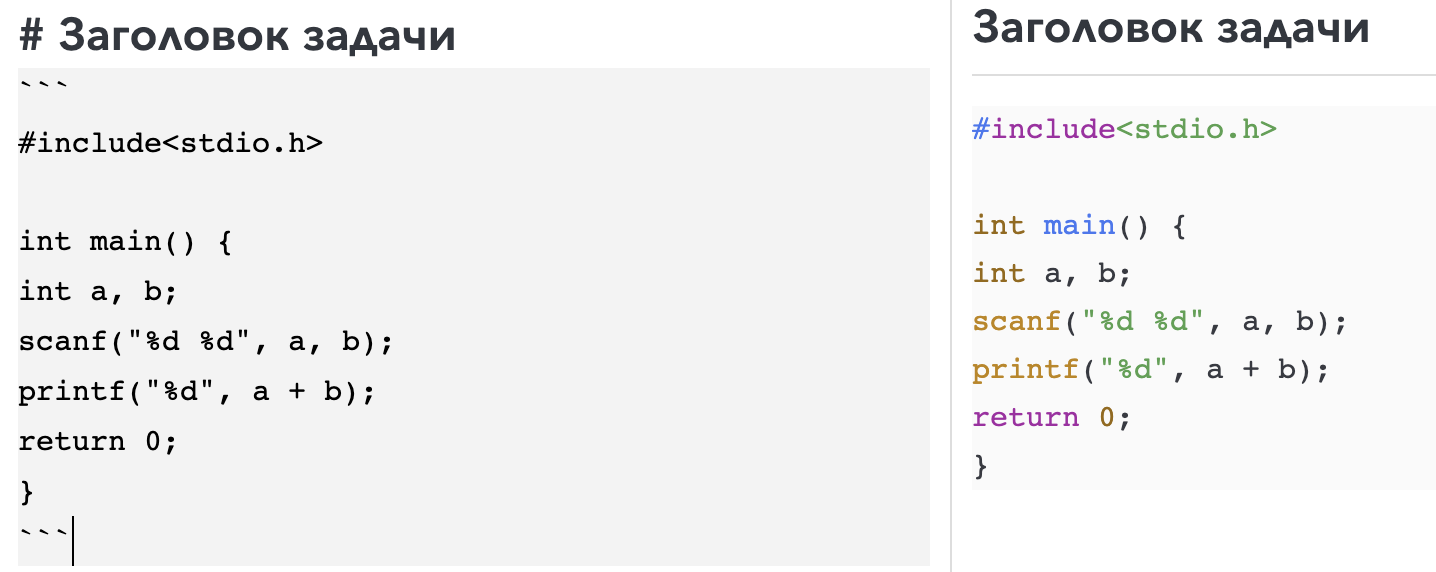
\includegraphics[width=0.75\linewidth]{src/10.png}
        \caption{Выделение кода}
    \end{figure}

    Прикрепить к заметке документ
    \begin{figure}[H]
        \centering
        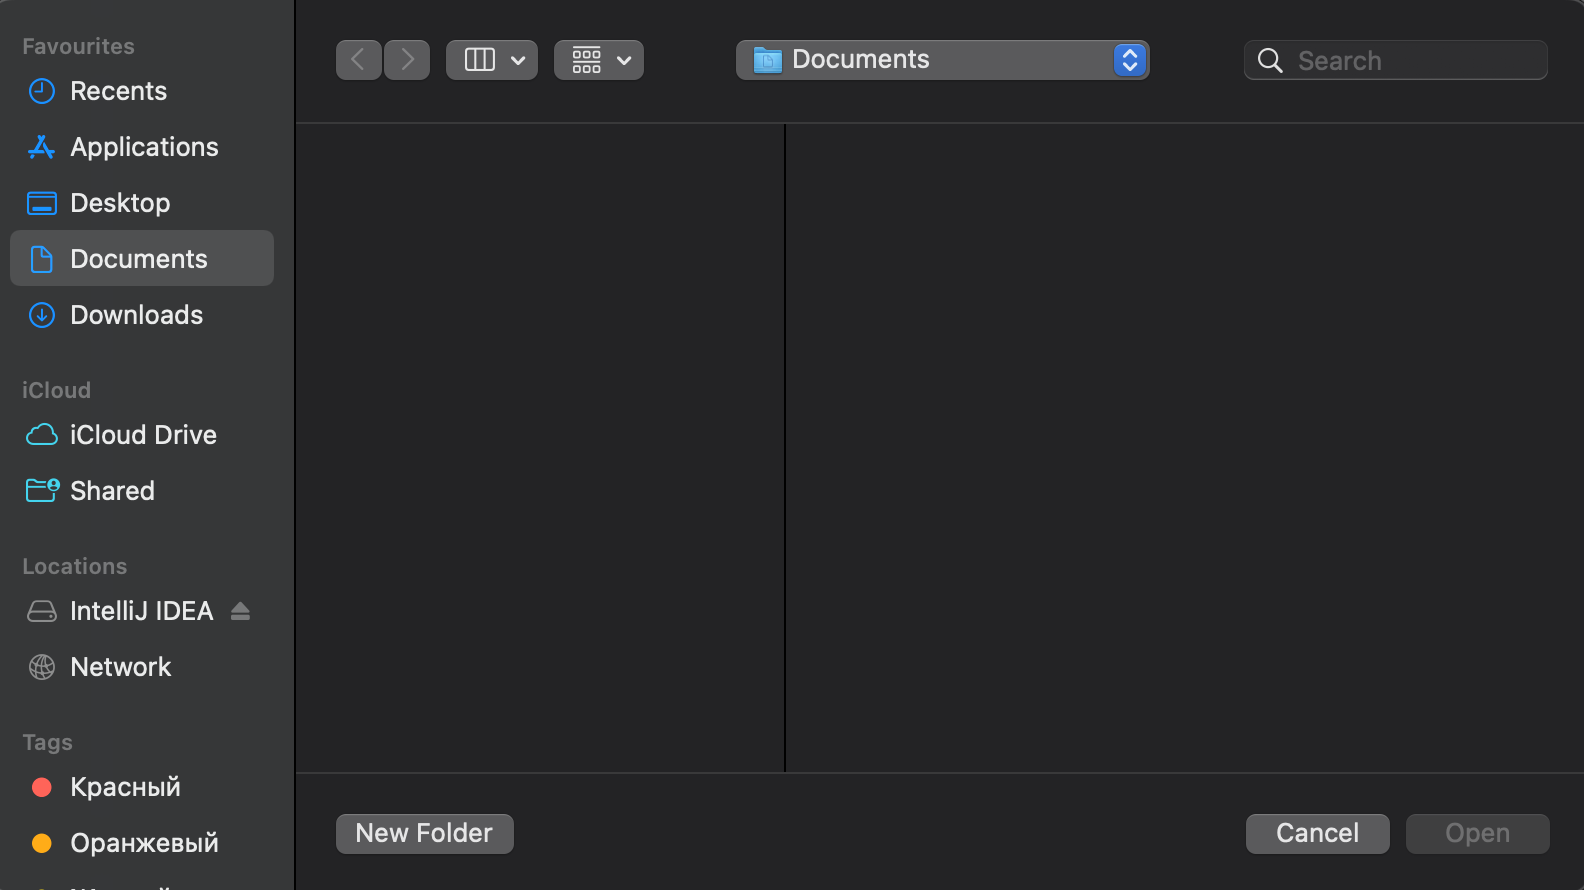
\includegraphics[width=0.75\linewidth]{src/11.png}
        \caption{Документ}
    \end{figure}

    Создавать различные списки, в том числе, с подзадачами, которые можно пометить
    \begin{figure}[H]
        \centering
        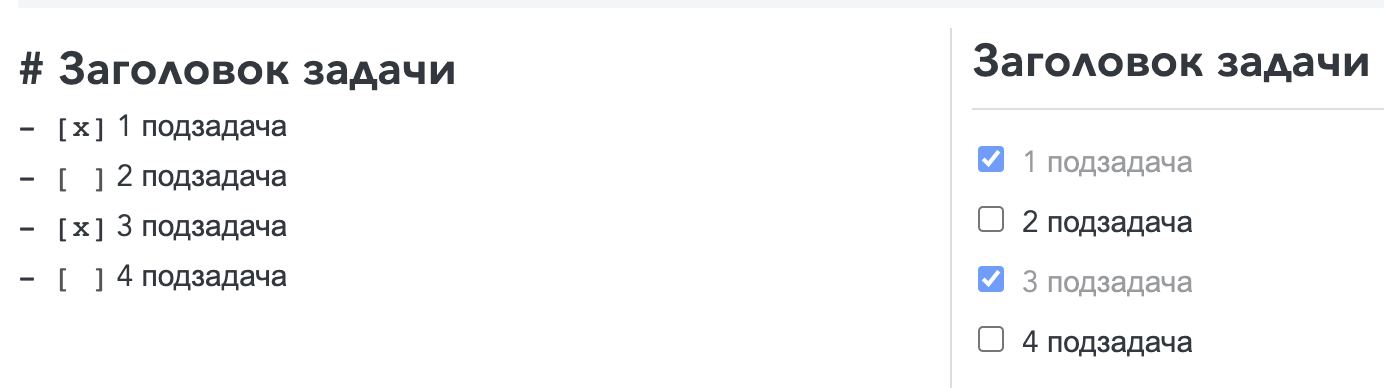
\includegraphics[width=0.75\linewidth]{src/12.png}
        \caption{Список подзадач}
    \end{figure}

    Может показаться, что это достаточно мало, но большая часть 
    функционала построена на возможностях markdown, а это немного выходит за рамки
    данного обзора.
    Поэтому я привел в пример основные возможности, которыми я пользуюсь в повседневной жизни.

    % page
    \newpage
    \section{Продвинутые настройки}
    \subsection{Настройки тесно связанные с базовым функционалом}
    Здесь мы можем настроить такие вещи как:
    \begin{itemize}
        \item Основной язык системы
        \item Формат даты и времени
        \item Путь к текстовому редактору и аргументы его запуска
        \item Размер документа на выходе
        \item Ориентация документа
        \item Версии хоткеев, среди которых можно также выбрать \textit{emacs} или \textit{vim}
    \end{itemize}
    \begin{figure}[H]
        \centering
        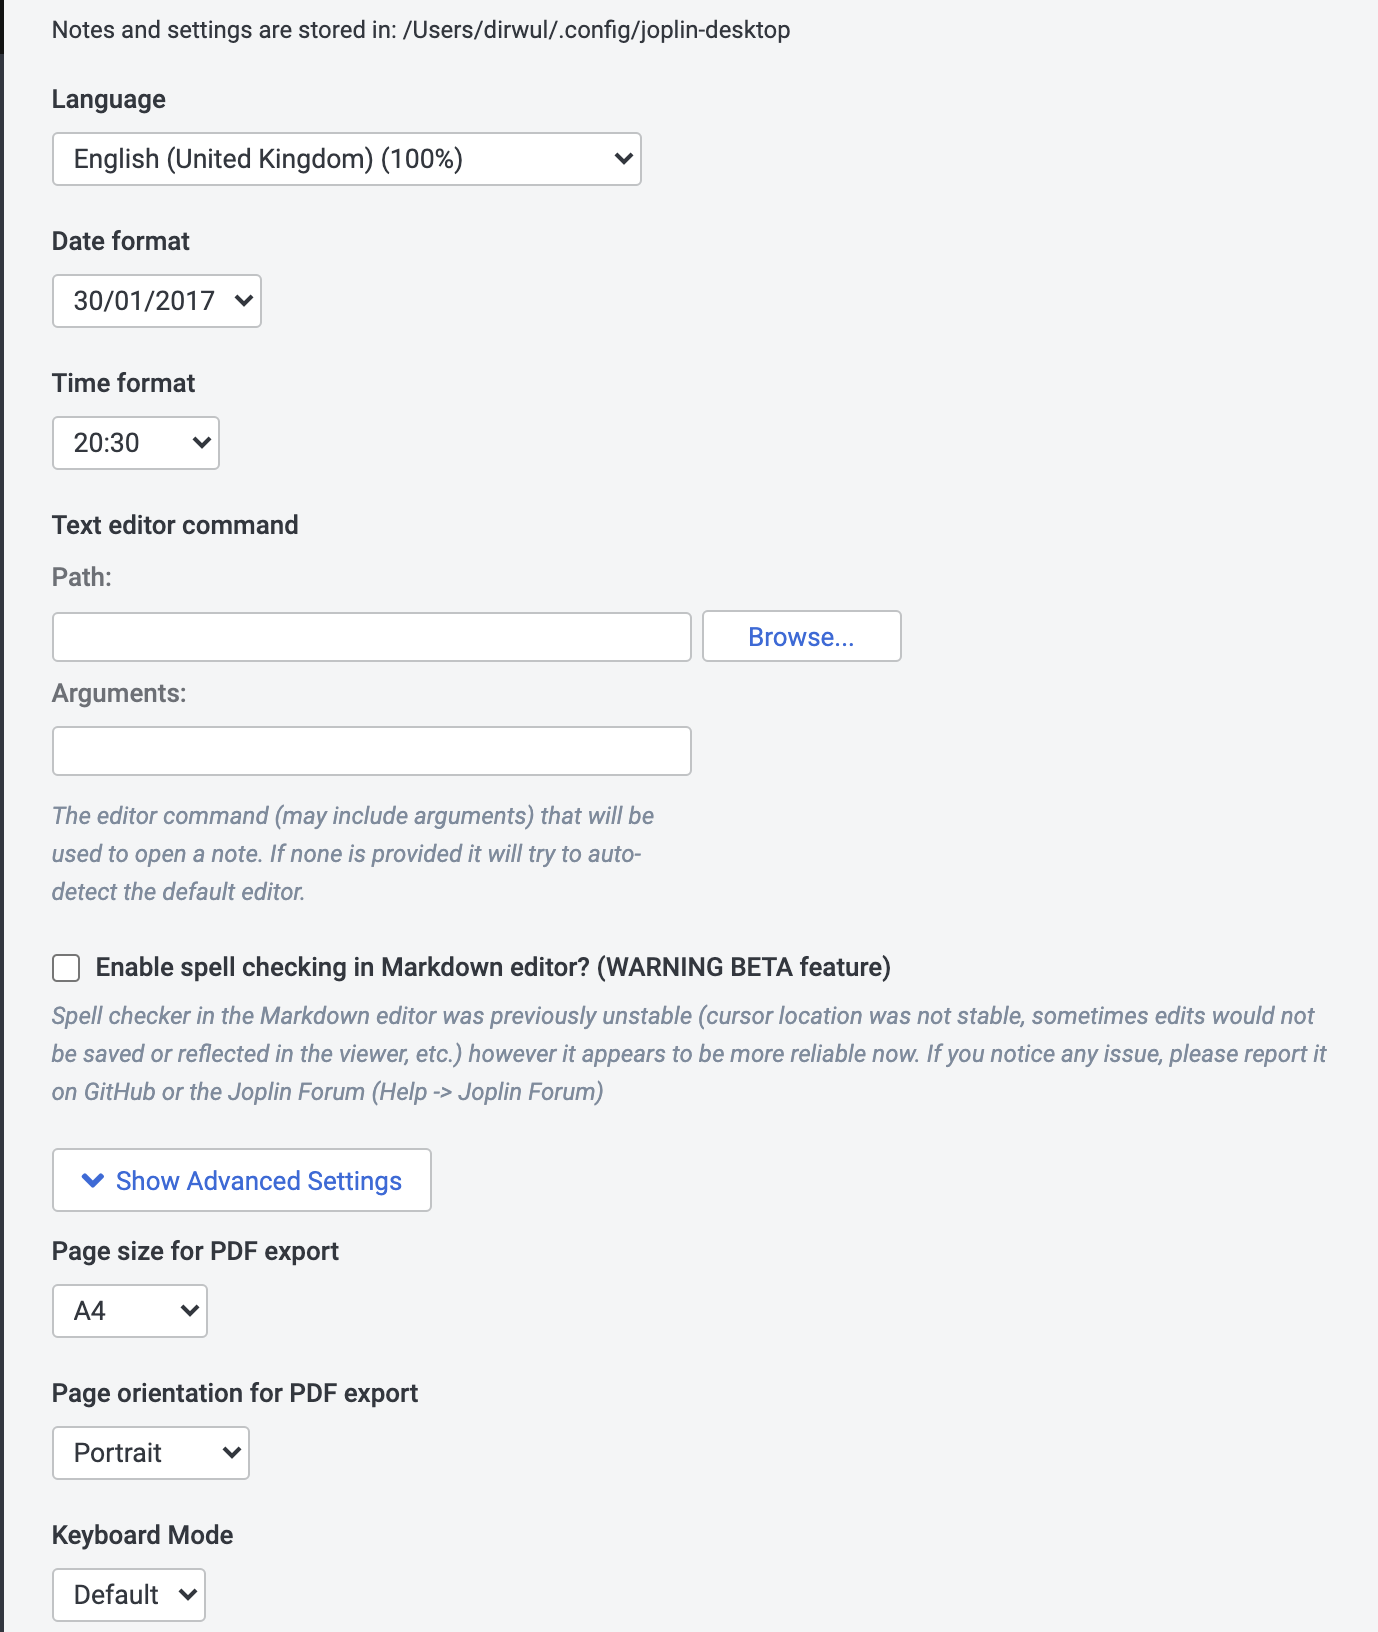
\includegraphics[width=0.75\linewidth]{src/13.png}
        \caption{Общие настройки}
    \end{figure}

    \newpage
    \subsection{Синхронизация}
    В настройках синхронизации можно поменять также некоторые параметры:
    \begin{itemize}
        \item Место хранения наших заметок, включая сервера самого Joplin \textit{(dropbox/one drive/etc)}
        \item Промежуток синхронизации
        \item Прочие ньюансы синхронизации
    \end{itemize}
    \begin{figure}[H]
        \centering
        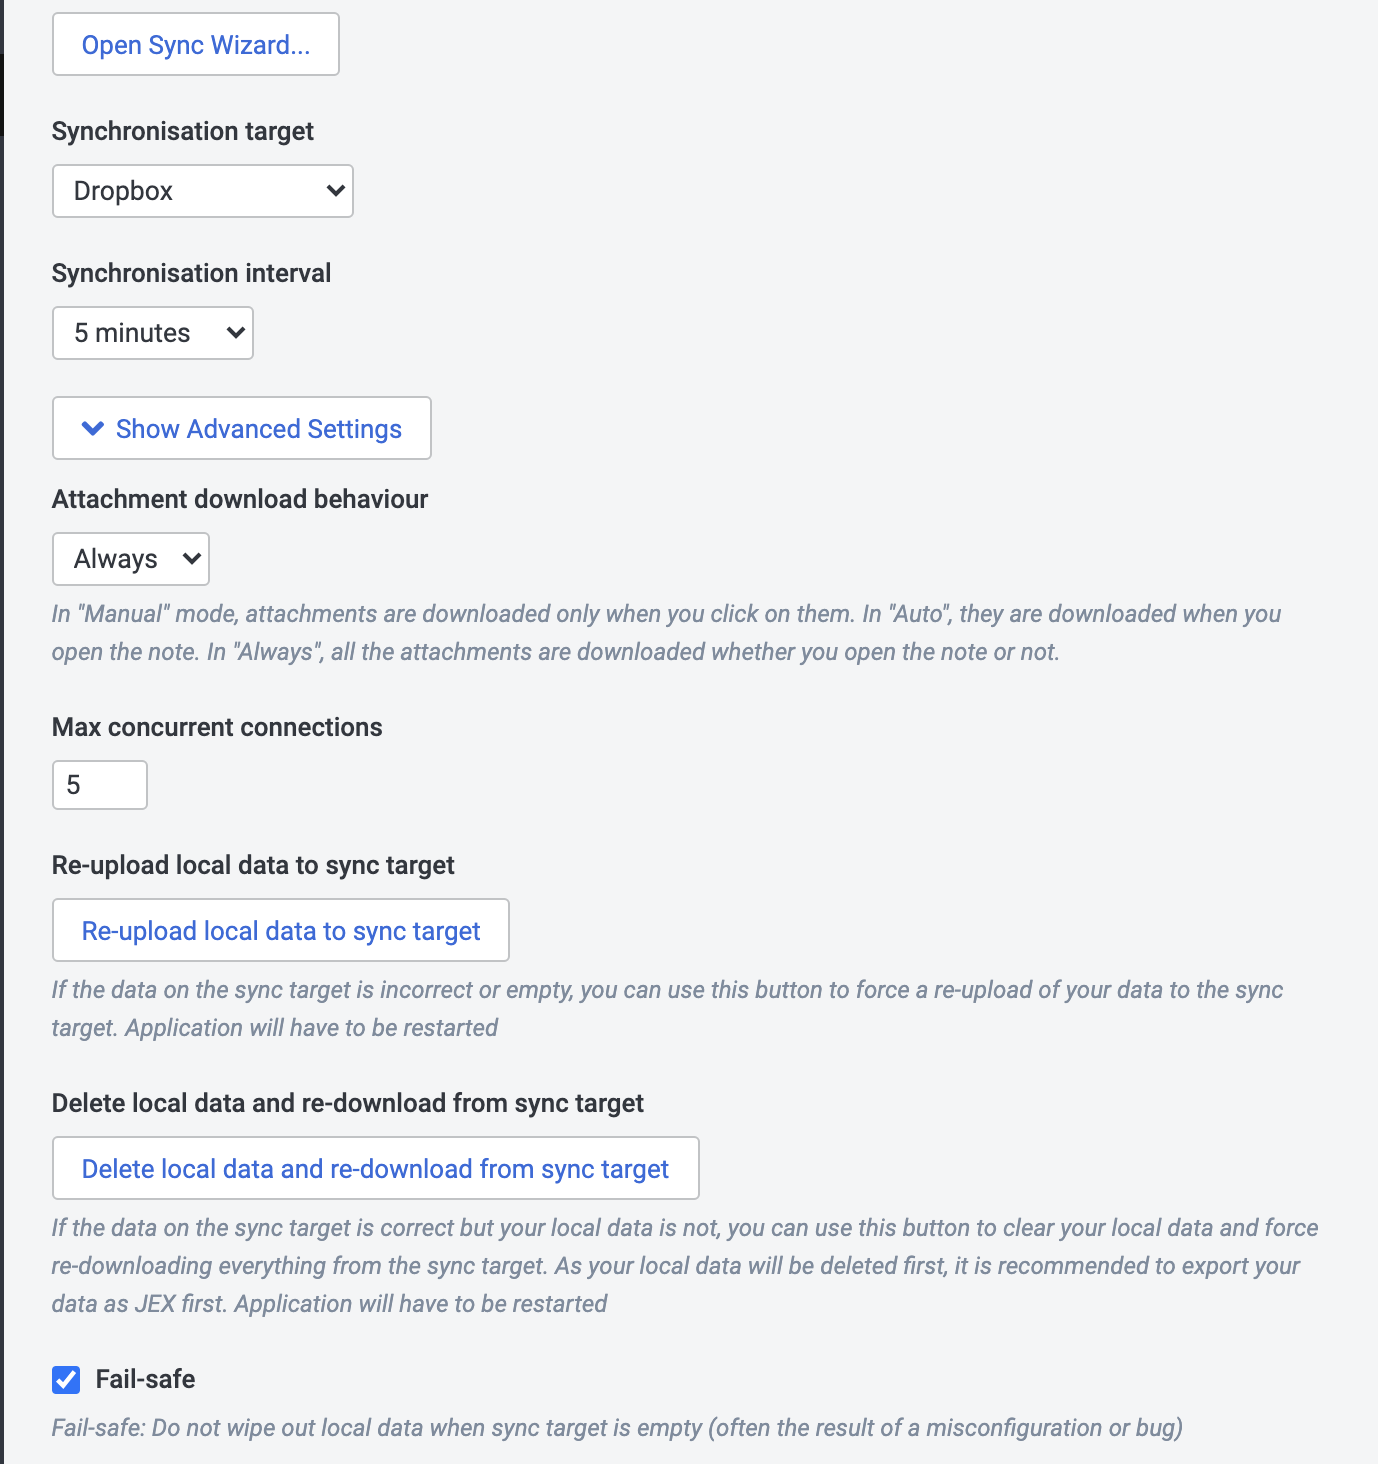
\includegraphics[width=0.75\linewidth]{src/14.png}
        \caption{Настройки синхронизации}
    \end{figure}

    \newpage
    \subsection{Настройки текстового редактора и отображения}
    \begin{itemize}
        \item Светлая/темная тема приложения
        \item Размер текста в редакторе
        \item Шрифт для различных видов текста
        \item Стили для markdown и html \textit{(да, Joplin так же поддерживает html нотации)}
    \end{itemize}
    \begin{figure}[H]
        \centering
        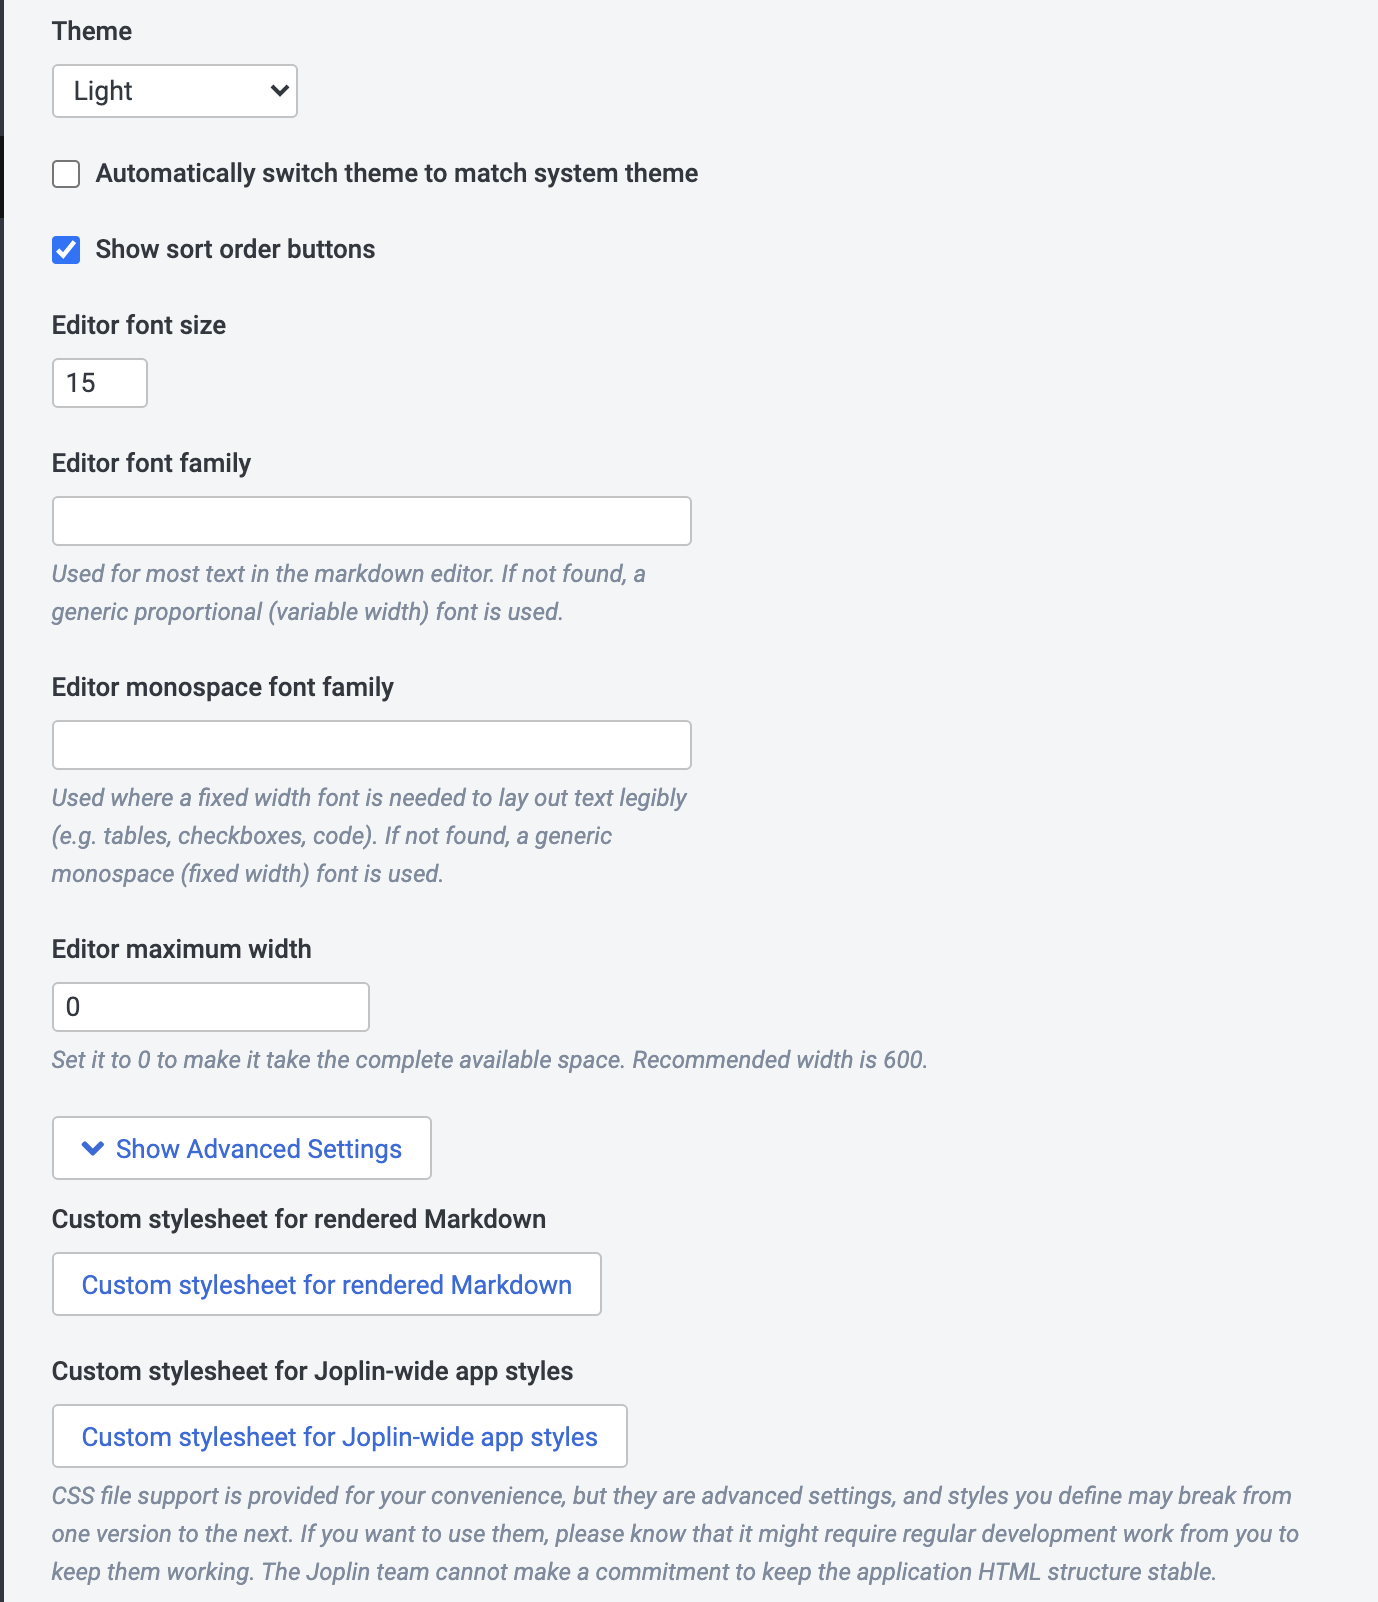
\includegraphics[width=0.75\linewidth]{src/15.png}
        \caption{Настройки текста}
    \end{figure}
    
    \newpage
    \subsection{Плагины}
    Одна из сильных сторон Joplin - возможность разрабатывать свои плагины или скачивать уже имеющиеся
    Секция настроек перебрасывает нас на репозиторий в гитхабе, в котором мы можем ознакомиться со всеми имеющимися на данный момент плагинами
    \begin{figure}[H]
        \centering
        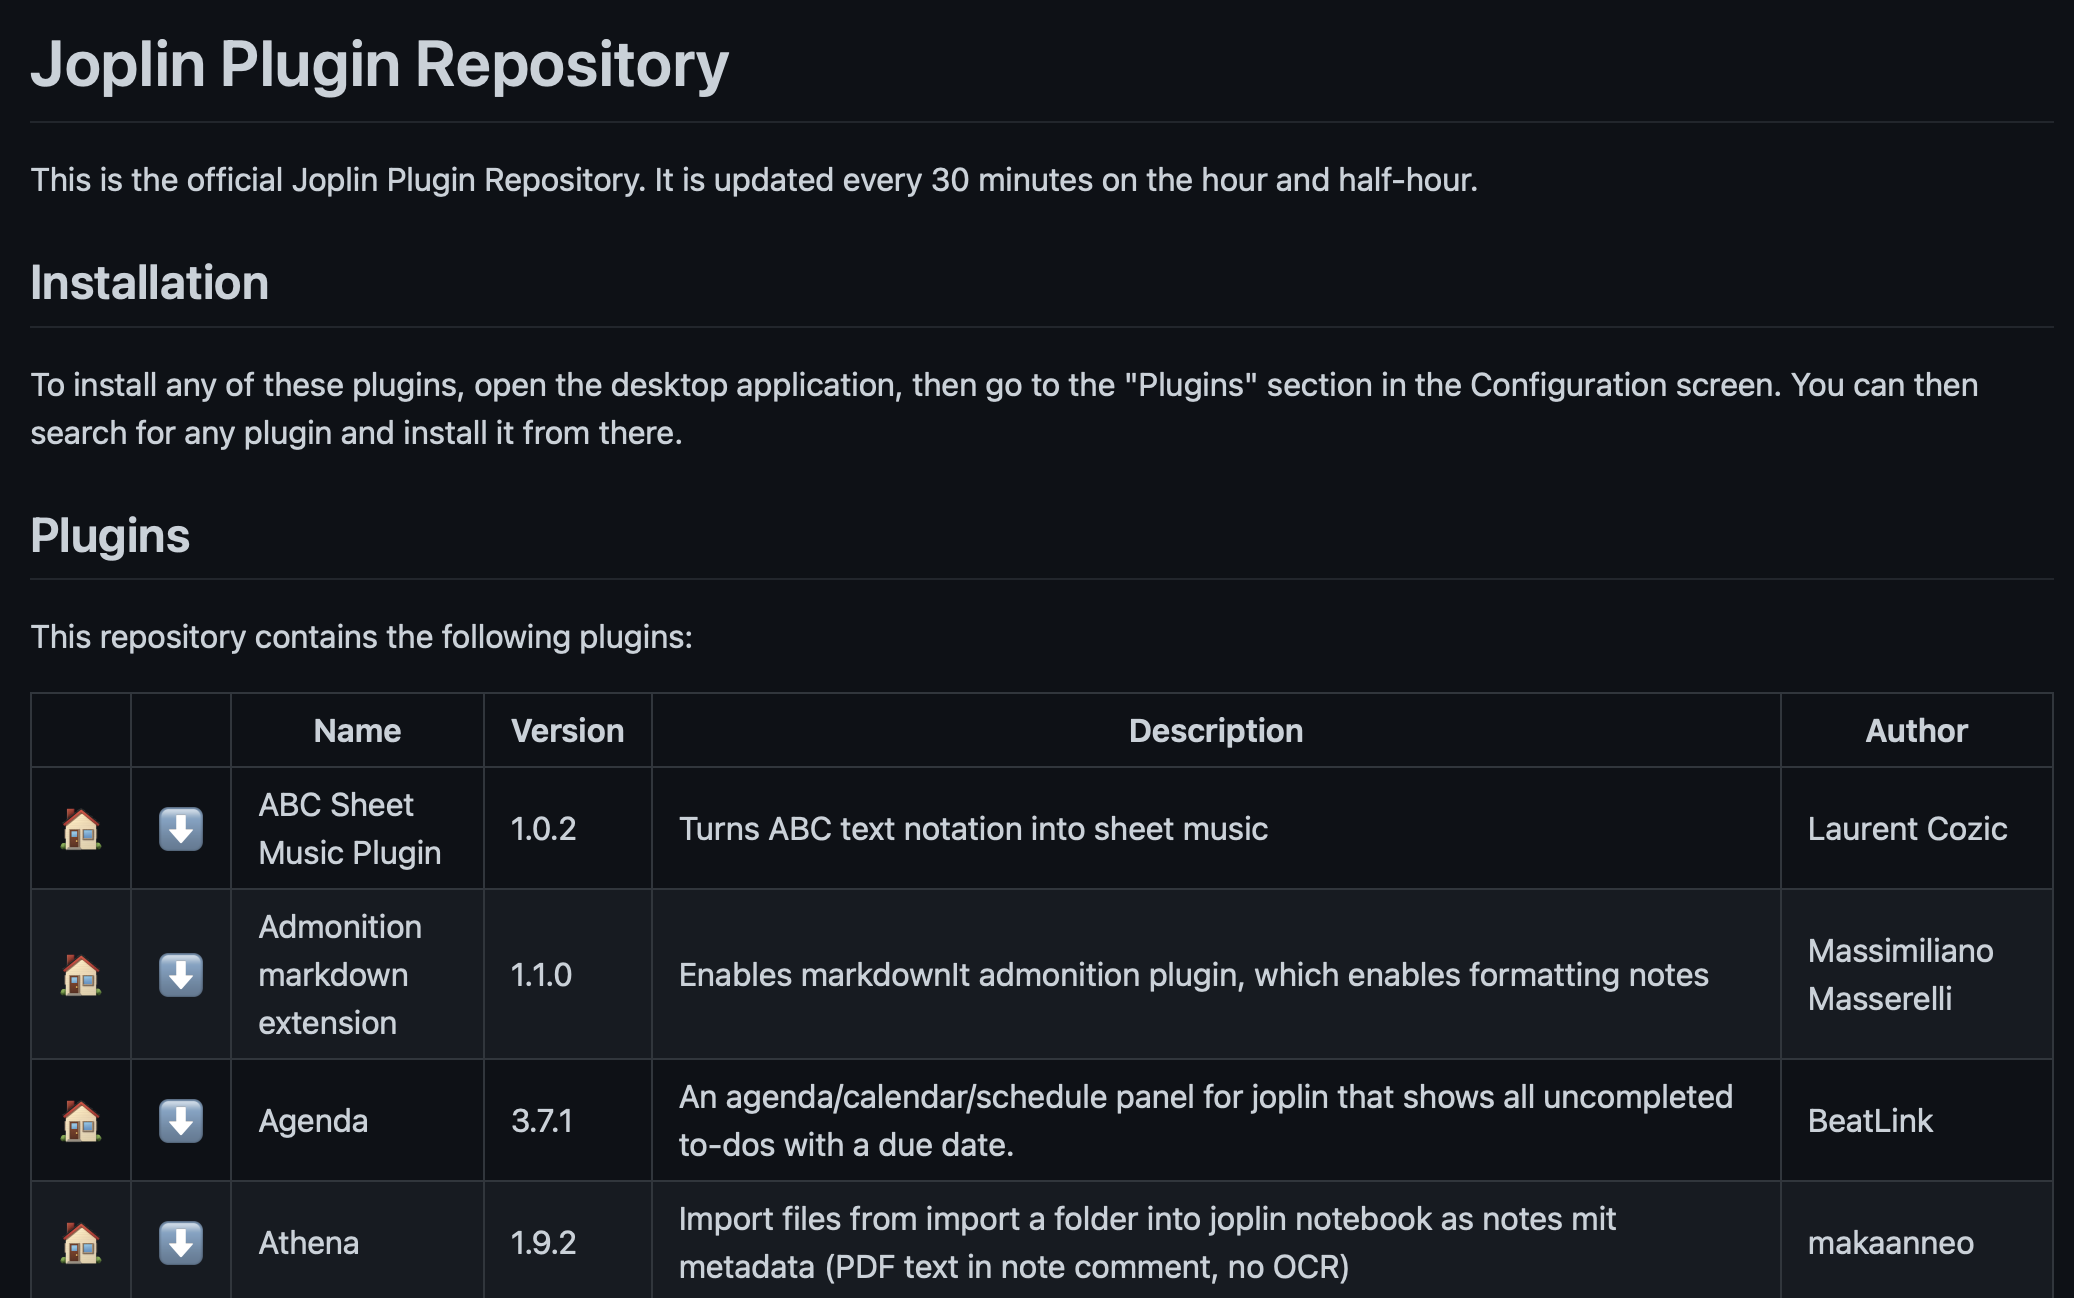
\includegraphics[width=0.75\linewidth]{src/16.png}
        \caption{Плагины на github}
    \end{figure}
    
    
    \subsection{Веб приложения}
    Так же у Joplin есть синхронизация с вебом, что позволяет нам довольно быстро сохранять какие-либо заметки из веба, или наоборот, добавлять их в статью
    \begin{figure}[H]
        \centering
        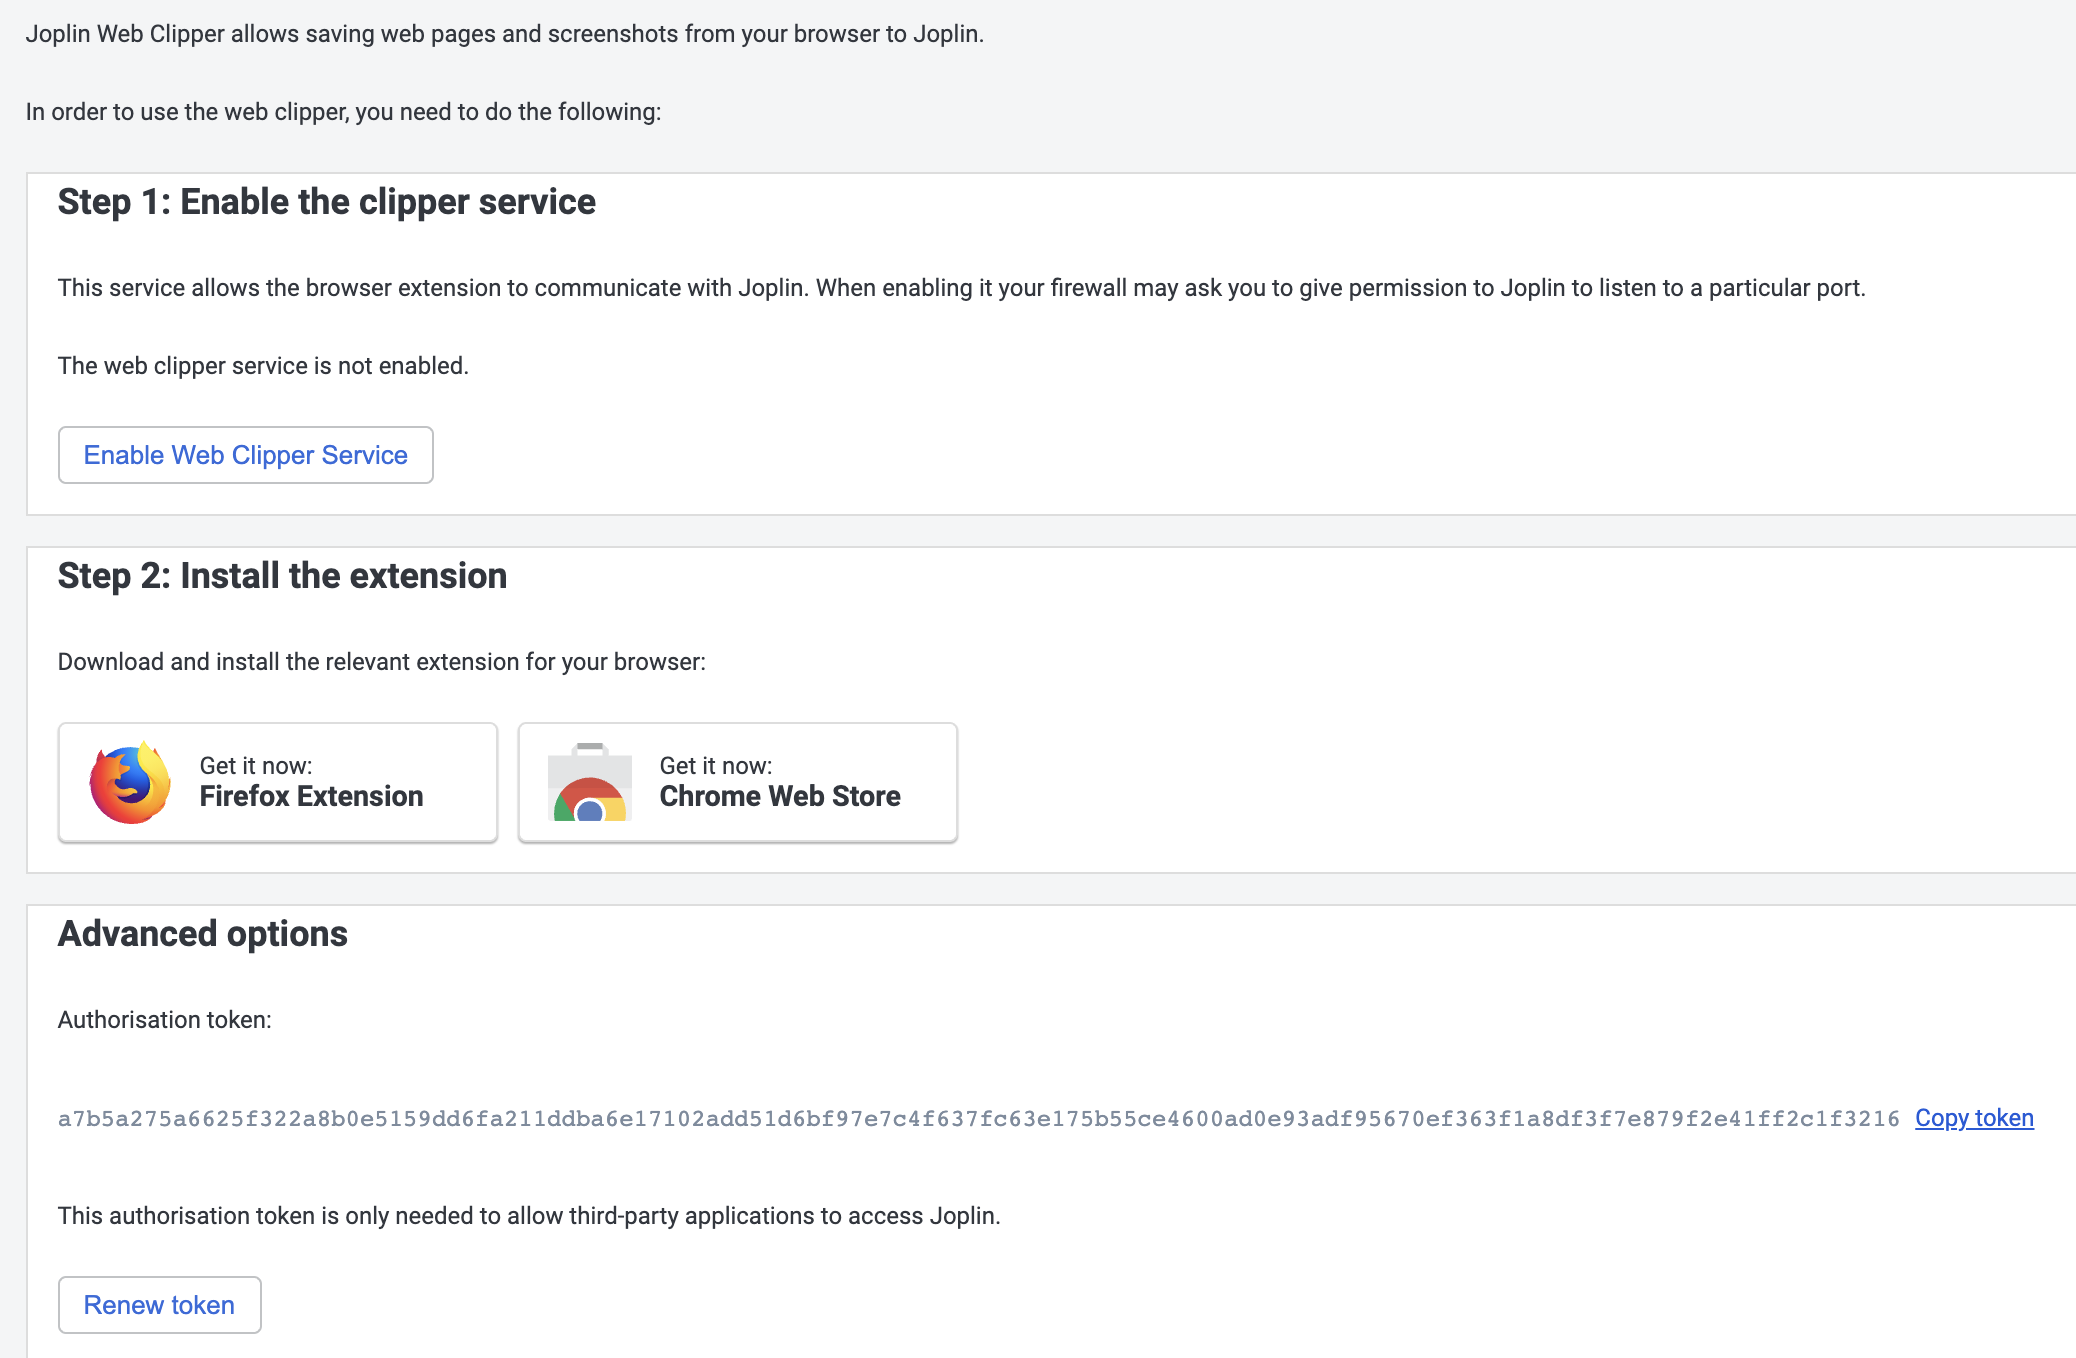
\includegraphics[width=0.75\linewidth]{src/17.png}
        \caption{Веб интеграция}
    \end{figure}
    
    \newpage
    \subsection{Хоткеи}
    Данная вкладка позволяет нам легко просмотреть все доступые в редакторе хоткеи и сценарии их использования с возможностью переназначить любой из них 
    \begin{figure}[H]
        \centering
        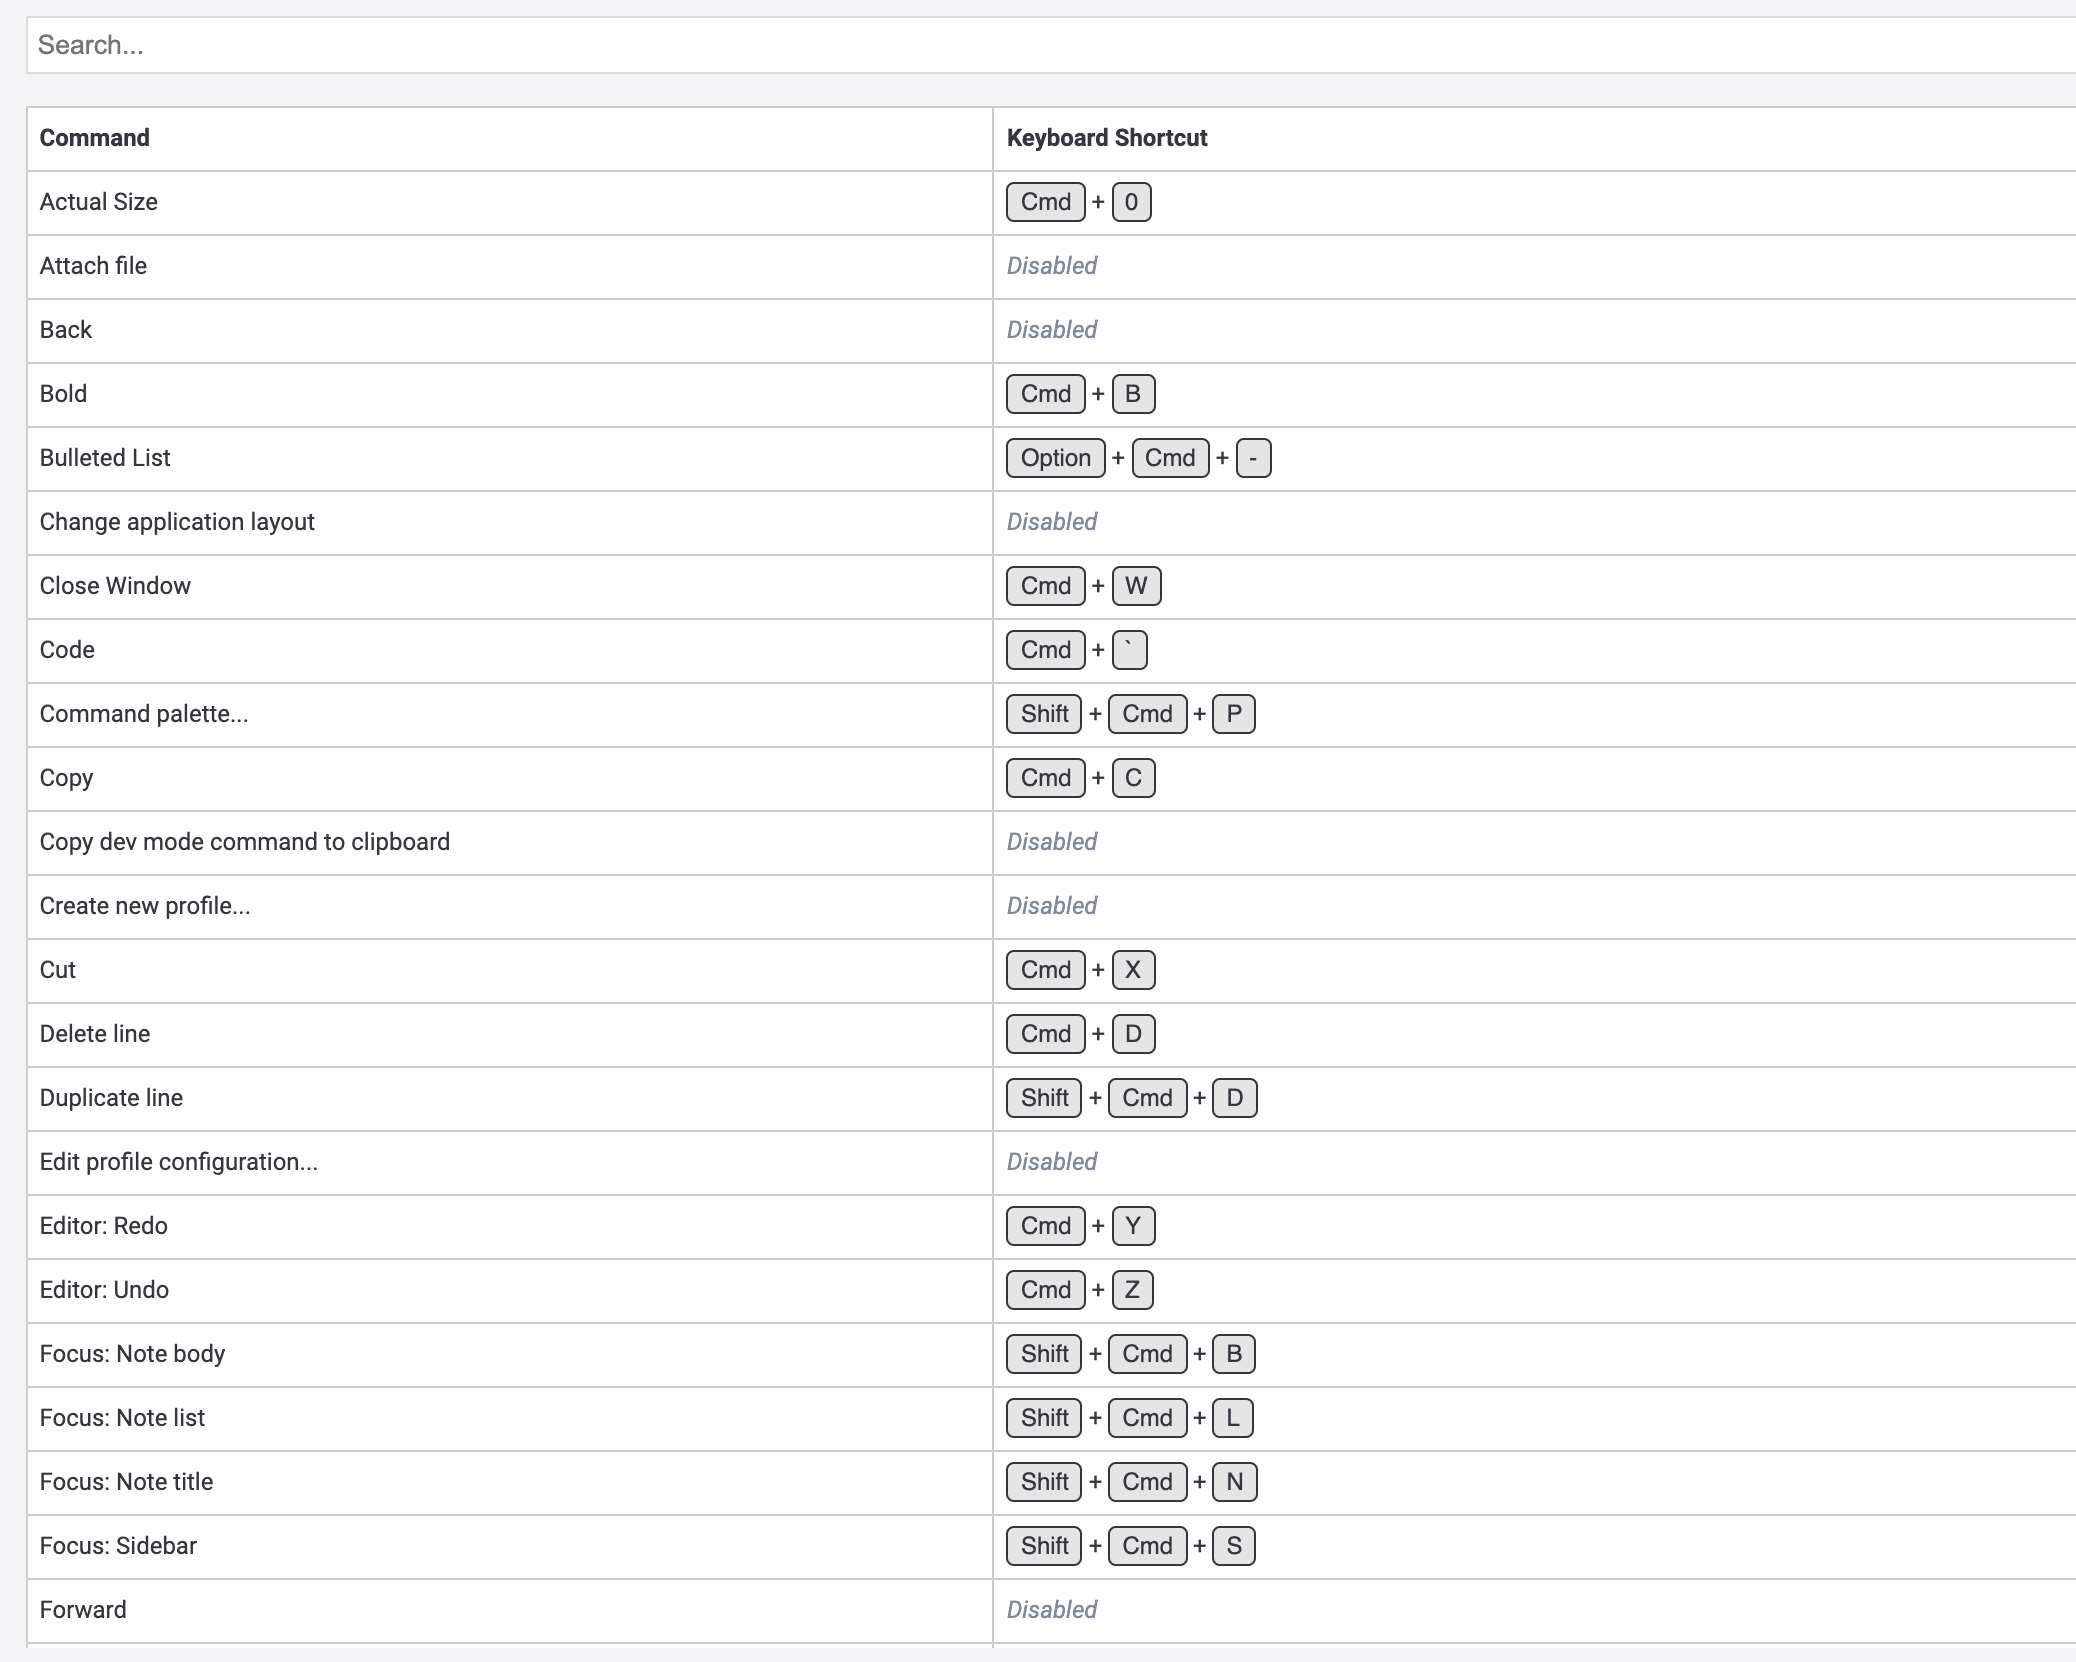
\includegraphics[width=0.75\linewidth]{src/18.png}
        \caption{Хоткеи}
    \end{figure}
    

\end{document}